\documentclass[10pt,twocolumn,letterpaper]{article}

\usepackage{cvpr}
\usepackage{times}
\usepackage{epsfig}
\usepackage{graphicx}
\usepackage{amsmath}
\usepackage{amssymb}
\usepackage{caption}
\usepackage{verbatim}
\usepackage{subcaption}
\usepackage{algorithm2e}
\usepackage{rotating}
\usepackage[space]{grffile}
\usepackage[font=small,skip=0pt]{caption}
%\DeclareMathOperator{\Tr}{Tr}
% Include other packages here, before hyperref.

% If you comment hyperref and then uncomment it, you should delete
% egpaper.aux before re-running latex.  (Or just hit 'q' on the first latex
% run, let it finish, and you should be clear).
\usepackage[breaklinks=true,bookmarks=false]{hyperref}
\graphicspath{ {figures/} }
% \cvprfinalcopy % *** Uncomment this line for the final submission

\def\cvprPaperID{2349} % *** Enter the CVPR Paper ID here
\def\httilde{\mbox{\tt\raisebox{-.5ex}{\symbol{126}}}}

% custom commands
\newcommand{\scream}[1]{{\color{red} \bf *** #1 ***}}

% Pages are numbered in submission mode, and unnumbered in camera-ready
%\ifcvprfinal\pagestyle{empty}\fi
\setcounter{page}{1}
\begin{document}

%%%%%%%%% TITLE
\title{Supplementary Material for the Paper ``Enriching Object Detection with\\2D-3D Registration and Continuous Viewpoint Estimation''}
%\title{Enrich Object Detection : 2D-3D registration and continuous viewpoint estimation}

% \author{First Author\\
% Institution1\\
% Institution1 address\\
% {\tt\small firstauthor@i1.org}
% % For a paper whose authors are all at the same institution,
% % omit the following lines up until the closing ``}''.
% % Additional authors and addresses can be added with ``\and'',
% % just like the second author.
% % To save space, use either the email address or home page, not both
% \and
% Second Author\\
% Institution2\\
% First line of institution2 address\\
% {\tt\small secondauthor@i2.org}
% }

\maketitle
%\thispagestyle{empty}

%%%%%%%%% BODY TEXT
We present qualitative results in the supplementary material for our paper
``Enriching Object Detection with 2D-3D Registration and Continuous Viewpoint
Estimation''.
% In Sect.~\ref{sec:3dobject}, we present detection result on qualitative results.

\section{3D Object Dataset}
\label{sect:3dobject}
We run our ensemble of NZ-WHO templates as a detector on 3D Object
dataset\cite{savarese07} without tuning and present detection average precision, average
viewpoint precision, viewpoint confusion matrix and mean precision in pose
estimation. See Fig.~\ref{fig:3dobject_ap}

Most of the error in viewpoint estimation come from frontal and back views

\begin{figure}[h]
  \centering
  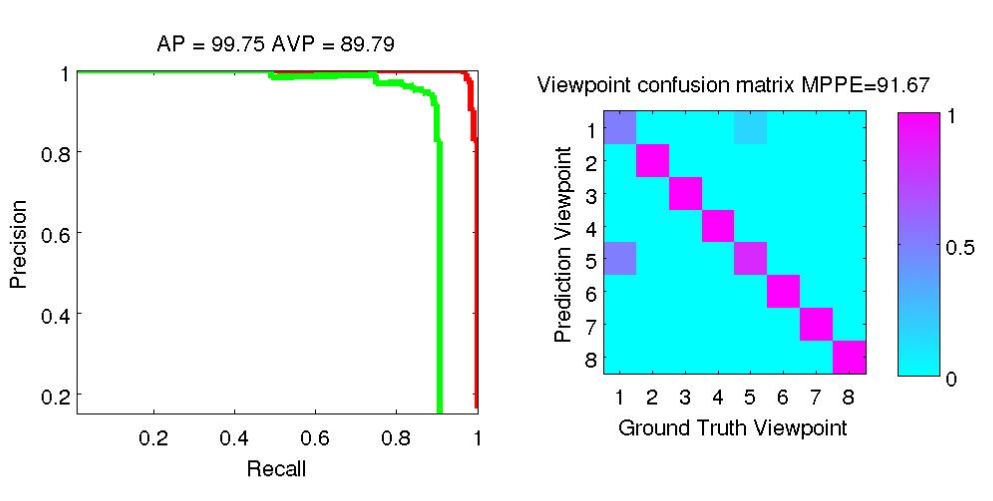
\includegraphics[width=0.99\linewidth]{supp/car_ap_3dobject_tight.png}\\
  \vspace{-5pt}
    (a) Car\\
  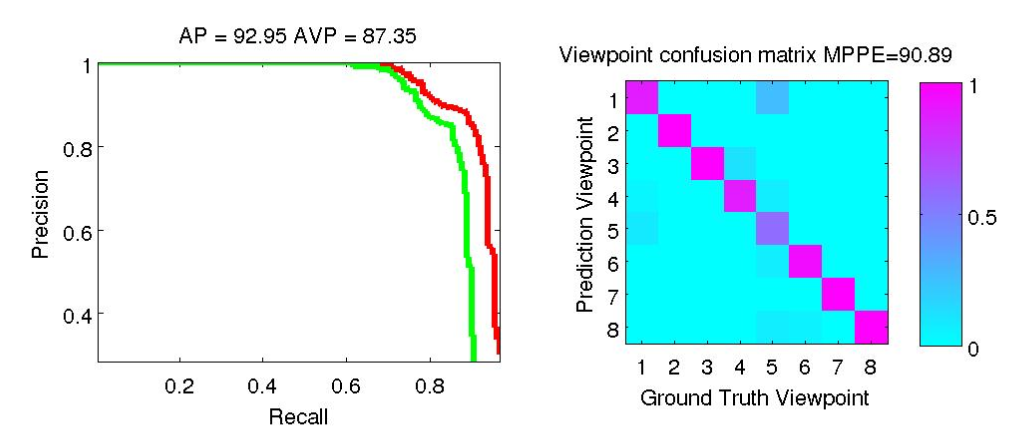
\includegraphics[width=0.99\linewidth]{supp/bicycle_ap_3dobject_tight.png}\\
  \vspace{-5pt}
    (b) Bicycle\\
  \caption{Detection and pose estimation on 3D Object dataset car category (top) and bicycle category (bottom).
  Average Precision (red) and Average Viewpoint Precision (green) (left)
  Viewpoint confusion table and MPPE (right), Viewpoint index 1 is front, index 2 is
  front-right, \dots index 8 is front-left. }
  \label{fig:3dobject_ap}
\end{figure}

We put successful car detection results on Fig.~\ref{fig:3dobject_car_good} and
failure cases on Fig.~\ref{fig:3dobject_car_bad}. And for bicycle, successful
bicycle detection results are on Fig.~\ref{fig:3dobject_bicycle_good} and
failure cases on Fig.~\ref{fig:3dobject_bicycle_bad}.

\begin{figure*}[h]
\setlength\tabcolsep{1pt}
\centering
\begin{tabular}{|c|c|}
  \hline
  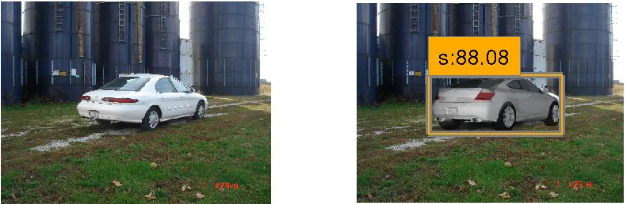
\includegraphics[width=0.40\linewidth]{supp/car32.png} &
  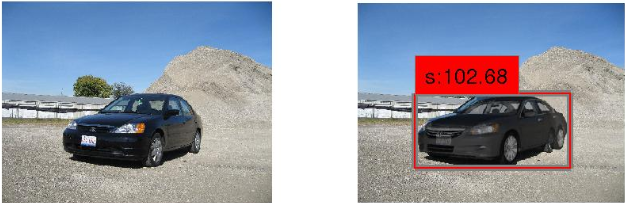
\includegraphics[width=0.40\linewidth]{supp/car26.png} \\
  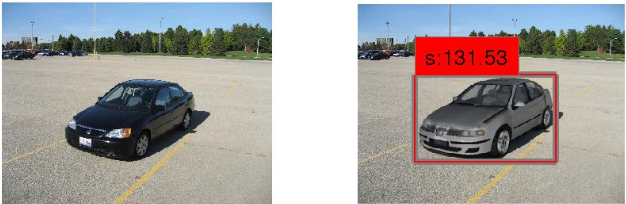
\includegraphics[width=0.40\linewidth]{supp/car29.png} & 
  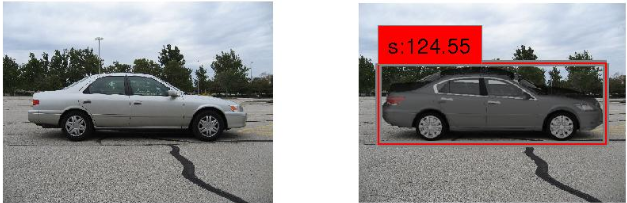
\includegraphics[width=0.40\linewidth]{supp/car10.png} \\
  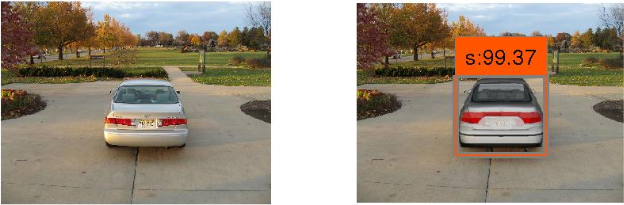
\includegraphics[width=0.40\linewidth]{supp/car1.png} &
  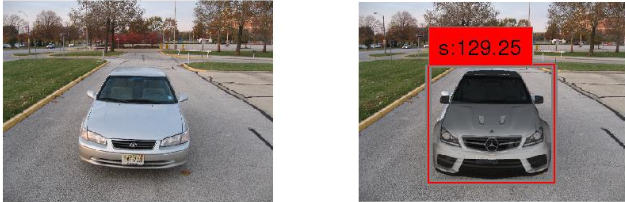
\includegraphics[width=0.40\linewidth]{supp/car8.png} \\
  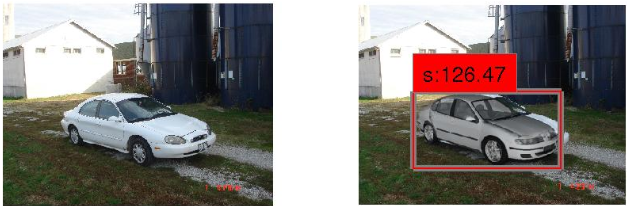
\includegraphics[width=0.40\linewidth]{supp/car20.png} & 
  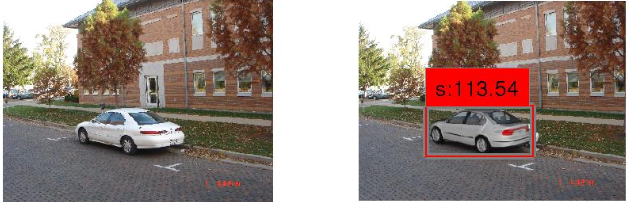
\includegraphics[width=0.40\linewidth]{supp/car31.png} \\
%   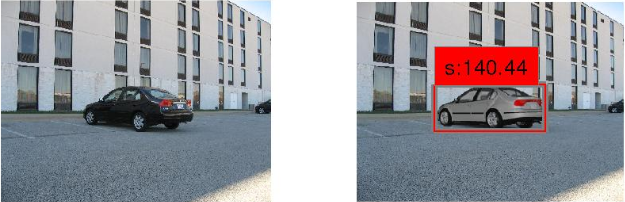
\includegraphics[width=0.40\linewidth]{supp/car33.png} & 
  \hline
  \end{tabular}
\caption{Successful detection results on 3D Object dataset car
category. In each column, original image (left) and detection result overlaid on
top (right).}% with a bounding box and corresponding confidence score (right).}
  \label{fig:3dobject_car_good}
\end{figure*}

\begin{figure*}[h]
\setlength\tabcolsep{1pt}
\centering
\begin{tabular}{|c|c|}
  \hline
  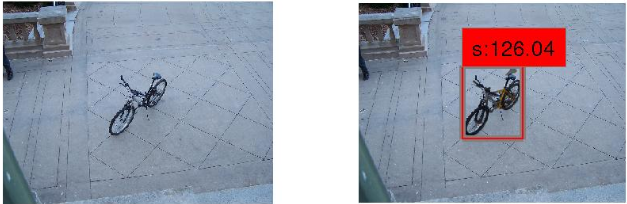
\includegraphics[width=0.40\linewidth]{supp/bicycle17.png} &
  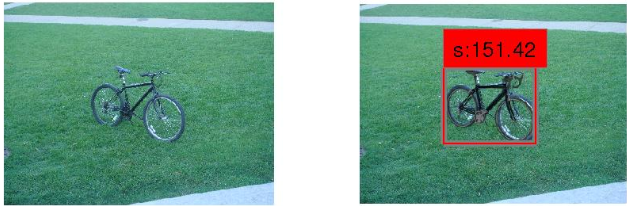
\includegraphics[width=0.40\linewidth]{supp/bicycle18.png} \\
  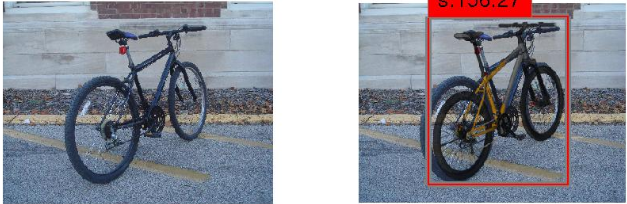
\includegraphics[width=0.40\linewidth]{supp/bicycle13.png} &
  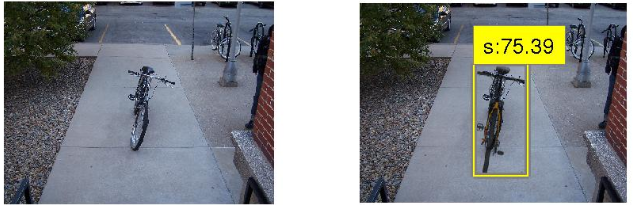
\includegraphics[width=0.40\linewidth]{supp/bicycle9.png} \\
  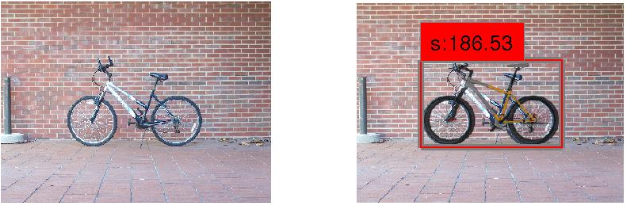
\includegraphics[width=0.40\linewidth]{supp/bicycle16.png} &
  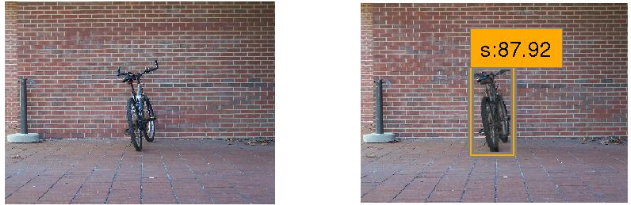
\includegraphics[width=0.40\linewidth]{supp/bicycle12.png} \\
  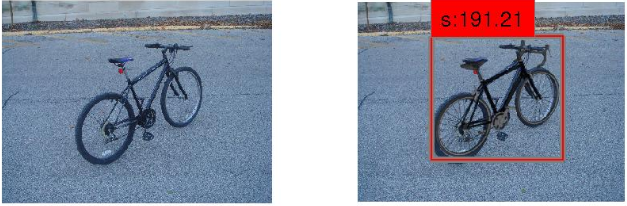
\includegraphics[width=0.40\linewidth]{supp/bicycle15.png} &
  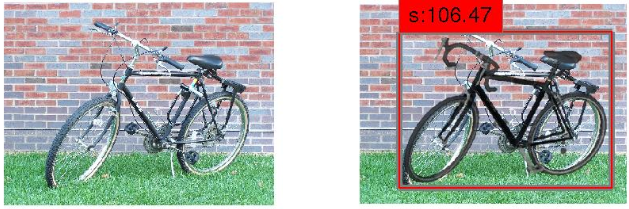
\includegraphics[width=0.40\linewidth]{supp/bicycle10.png} \\
  \hline
  \end{tabular}
\caption{Successful detection results on 3D Object dataset car
classes. In each column, original image (left) and detection result overlaid on
top (right).}% with a bounding box and corresponding confidence score (right).}
  \label{fig:3dobject_bicycle_good}
\end{figure*}


\begin{figure*}[h]
\setlength\tabcolsep{1pt}
\centering
\begin{tabular}{|c|c|}
  \hline
  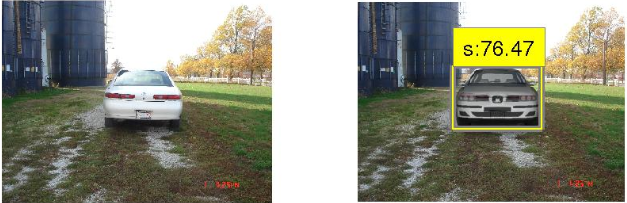
\includegraphics[width=0.40\linewidth]{supp/car13.png} &
  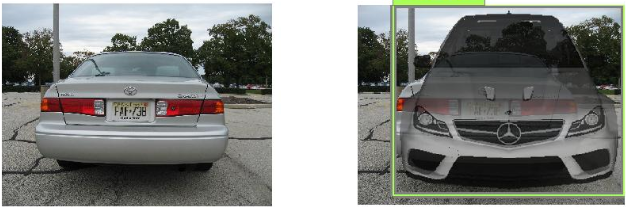
\includegraphics[width=0.40\linewidth]{supp/car30.png} \\ 
  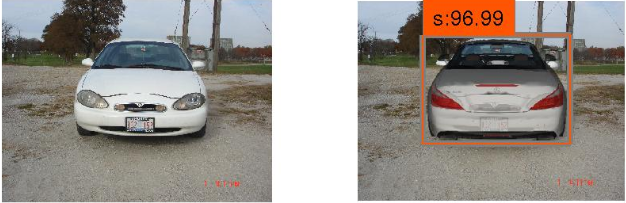
\includegraphics[width=0.40\linewidth]{supp/car18.png} &
  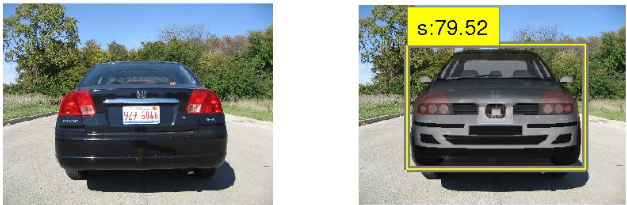
\includegraphics[width=0.40\linewidth]{supp/car25.png} \\
  \hline
  \end{tabular}
\caption{Failed pose estimation results on 3D Object dataset car and bike
classes. In each column, original image (left) and detection result overlaid on
top (right).}% with a bounding box and corresponding confidence score (right).}
  \label{fig:3dobject_car_bad}
\end{figure*}

\begin{figure*}[h]
\setlength\tabcolsep{1pt}
\centering
\begin{tabular}{|c|c|}
\hline 
  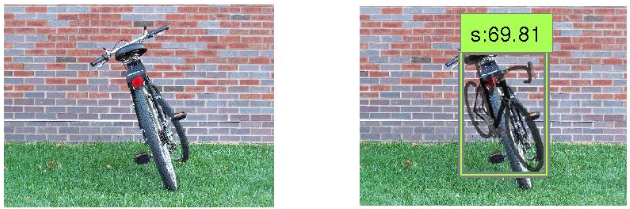
\includegraphics[width=0.40\linewidth]{supp/bicycle1.png} &
  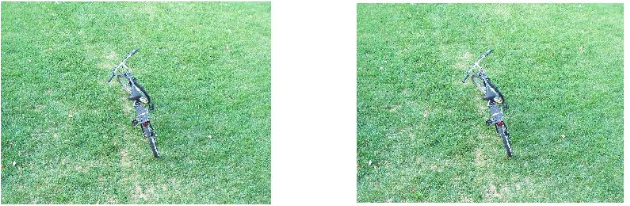
\includegraphics[width=0.40\linewidth]{supp/bicycle5.png} \\
  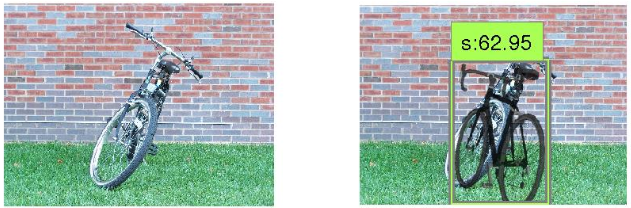
\includegraphics[width=0.40\linewidth]{supp/bicycle19.png} &
  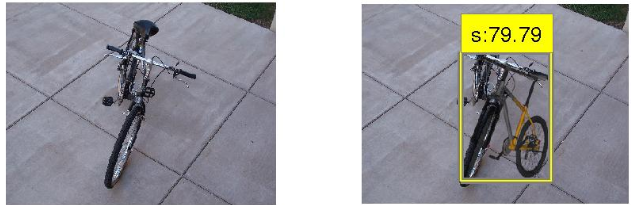
\includegraphics[width=0.40\linewidth]{supp/bicycle20.png} \\
\hline
\end{tabular}
\caption{Failed pose estimation results on 3D Object dataset car and bike
classes. In each column, original image (left) and detection result overlaid on
top (right).}% with a bounding box and corresponding confidence score (right).}
  \label{fig:3dobject_bicycle_bad}
\end{figure*}



\section{PASCAL3D+}

We run our ensemble of NZ-WHO templates as a detector on car
and bicycle classes in PASCAL3D+ dataset  \cite{Xiang14} and present detection average precision,
average viewpoint precision, viewpoint confusion matrix and mean precision in
pose estimation. See Fig.~\ref{fig:3dobject_ap}

For each of the proposal bounding box, we assumed that there is only one object and the object 
\begin{figure*}[h]
\setlength\tabcolsep{1pt}
\centering
\begin{tabular}{|cc|cc|}
  \hline
  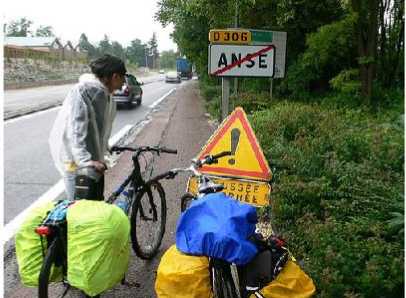
\includegraphics[width=0.24\linewidth]{supp/occlusion1.png} &
  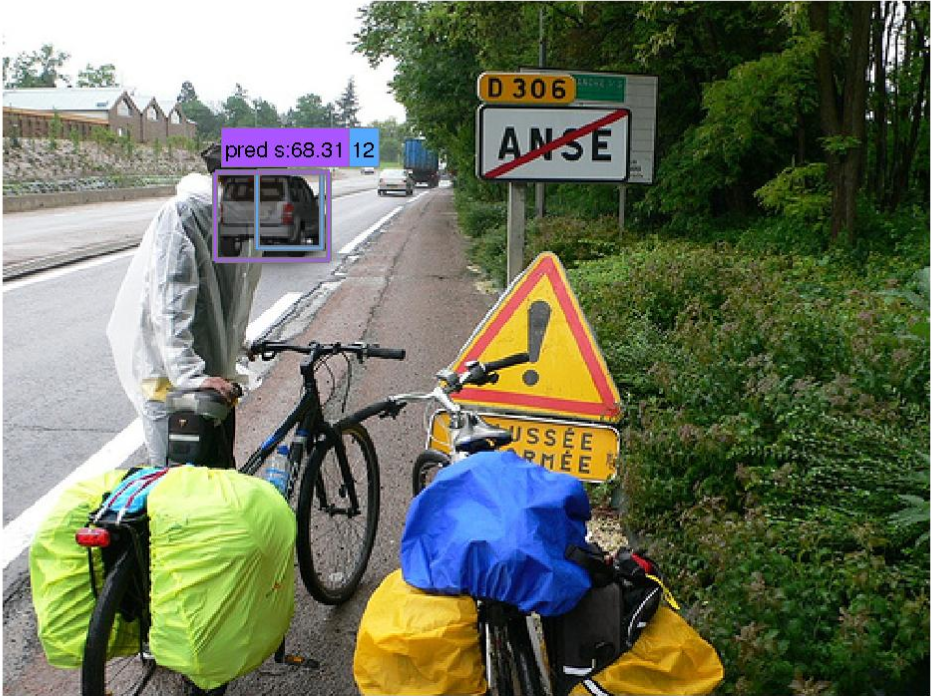
\includegraphics[width=0.24\linewidth]{supp/occlusion1b.png} & 
  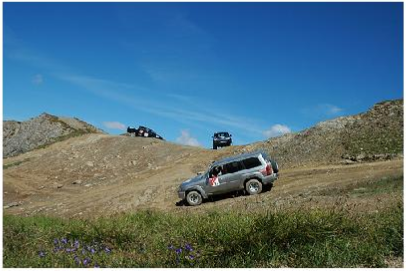
\includegraphics[width=0.24\linewidth]{supp/pas_car1a.png} &
  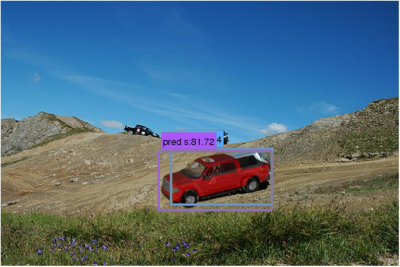
\includegraphics[width=0.24\linewidth]{supp/pas_car1b.png}  \\
  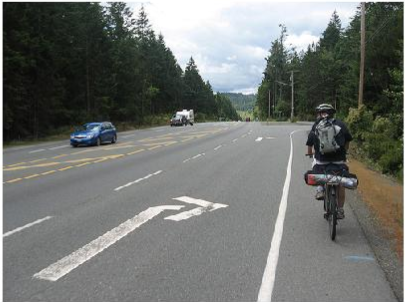
\includegraphics[width=0.24\linewidth]{supp/pas_car3a.png} &
  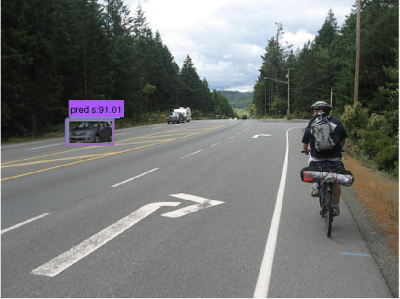
\includegraphics[width=0.24\linewidth]{supp/pas_car3b.png} & 
  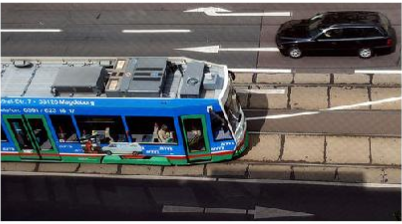
\includegraphics[width=0.24\linewidth]{supp/pas_car5a.png} &
  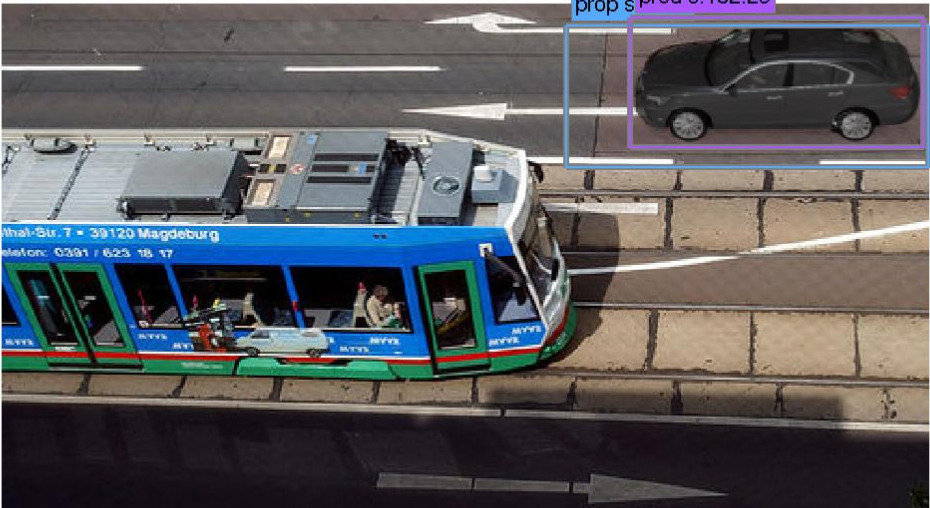
\includegraphics[width=0.24\linewidth]{supp/pas_car5b.png}  \\
  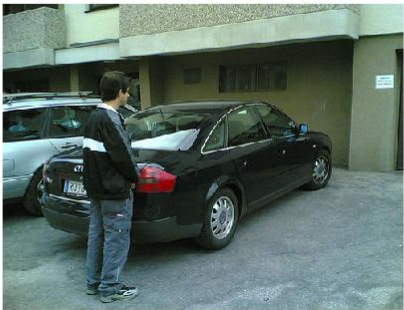
\includegraphics[width=0.24\linewidth]{supp/pas_car6a.png} &
  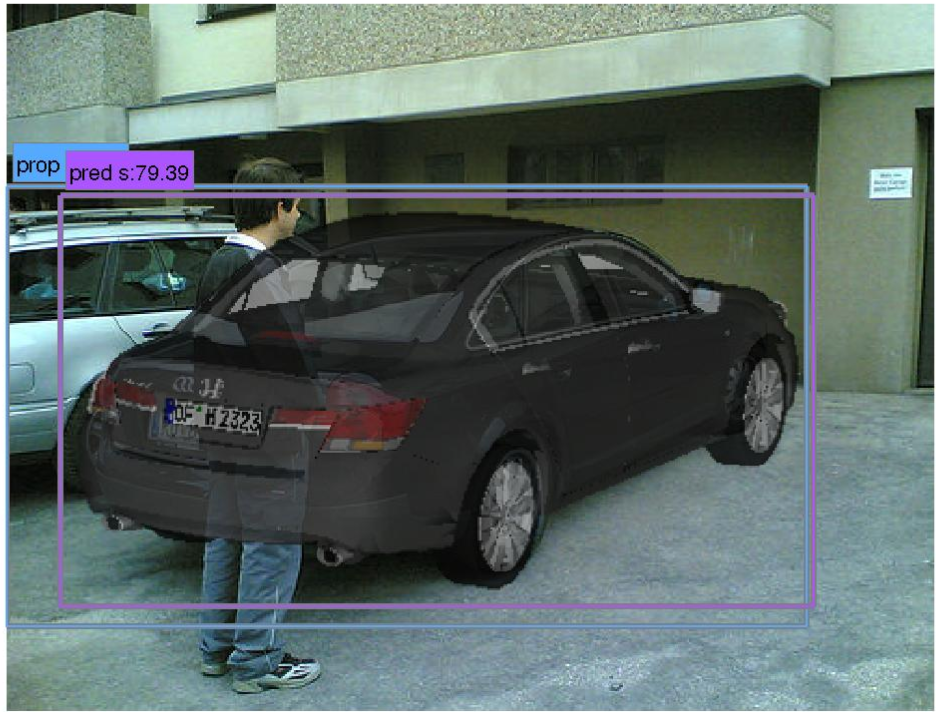
\includegraphics[width=0.24\linewidth]{supp/pas_car6b.png} & 
  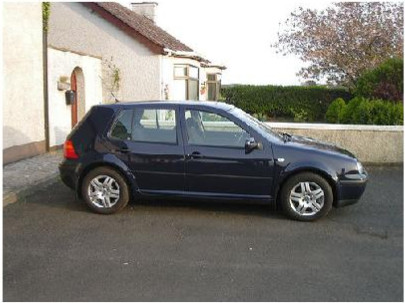
\includegraphics[width=0.24\linewidth]{supp/pas_car7a.png} &
  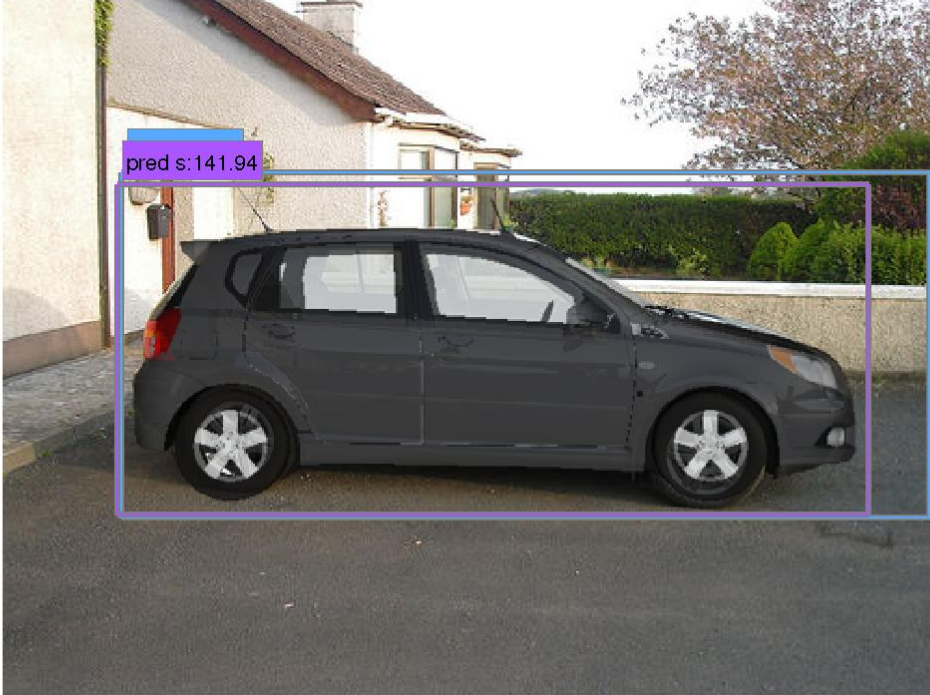
\includegraphics[width=0.24\linewidth]{supp/pas_car7b.png}  \\
  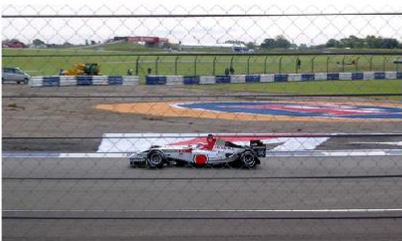
\includegraphics[width=0.24\linewidth]{supp/pas_car10a.png} &
  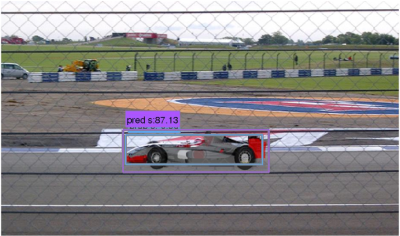
\includegraphics[width=0.24\linewidth]{supp/pas_car10b.png} & 
  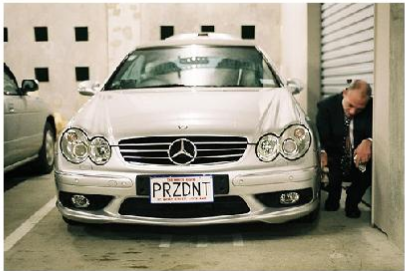
\includegraphics[width=0.24\linewidth]{supp/pas_car16a.png} &
  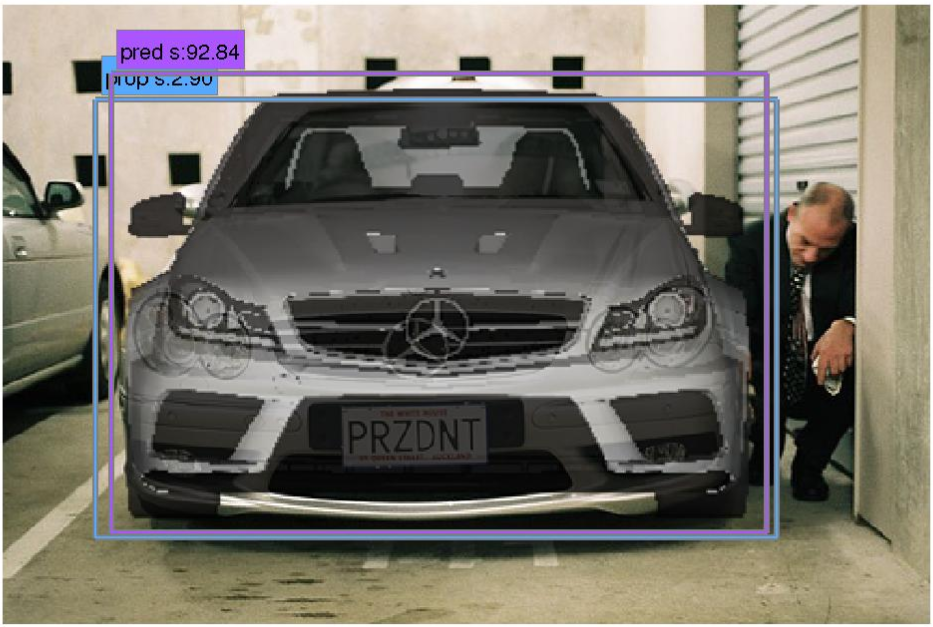
\includegraphics[width=0.24\linewidth]{supp/pas_car16b.png}  \\
  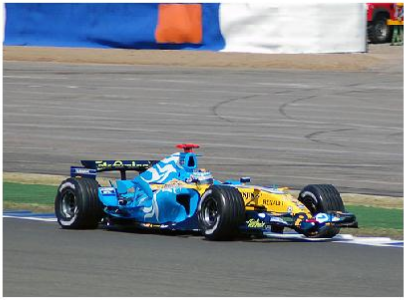
\includegraphics[width=0.24\linewidth]{supp/pas_car17a.png} &
  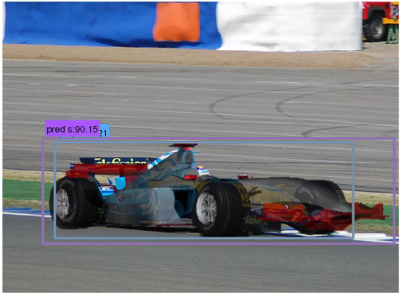
\includegraphics[width=0.24\linewidth]{supp/pas_car17b.png} & 
  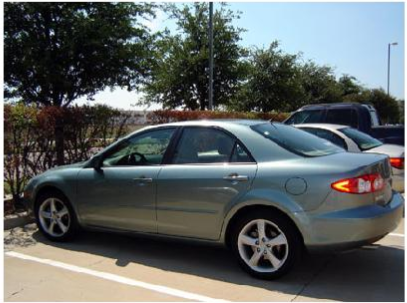
\includegraphics[width=0.24\linewidth]{supp/pas_car19a.png} &
  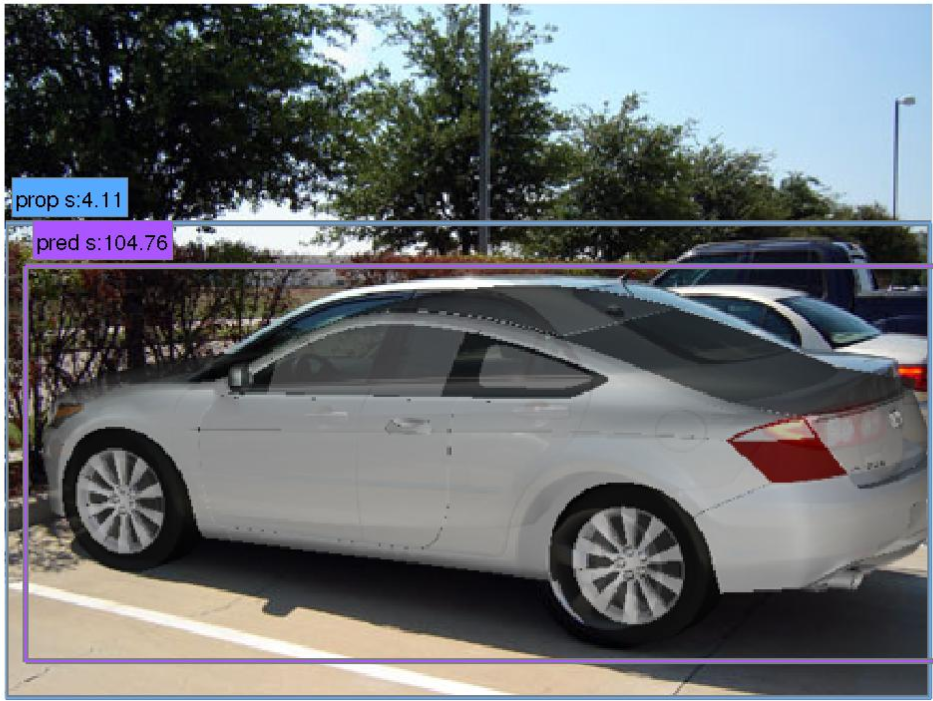
\includegraphics[width=0.24\linewidth]{supp/pas_car19b.png} \\
  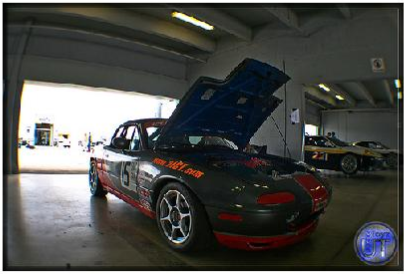
\includegraphics[width=0.24\linewidth]{supp/pas_car21a.png} &
  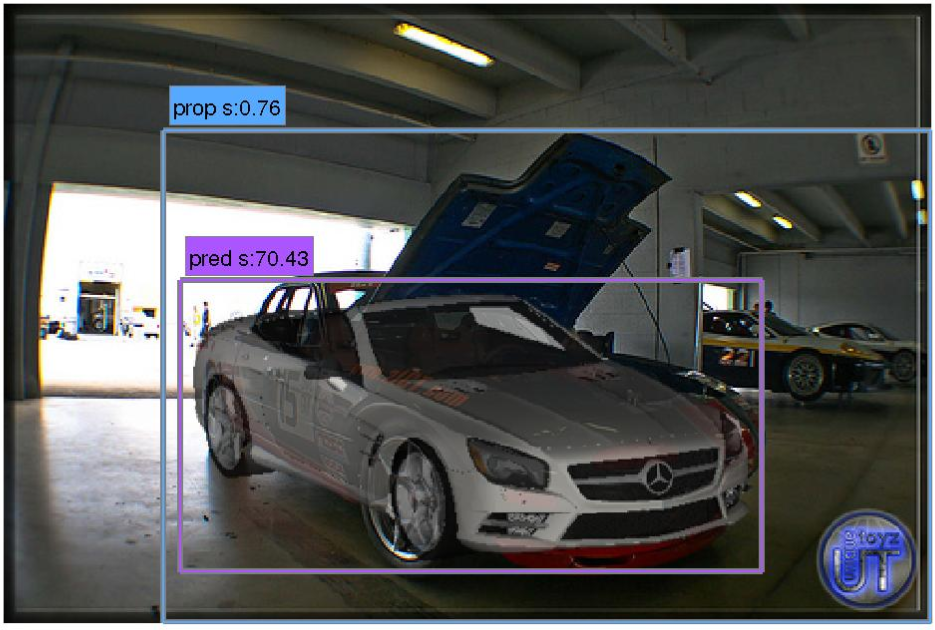
\includegraphics[width=0.24\linewidth]{supp/pas_car21b.png} & 
  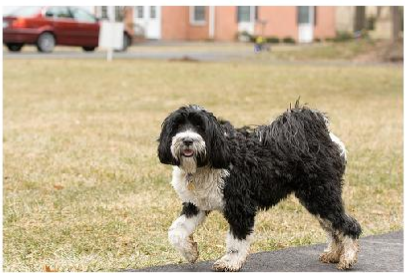
\includegraphics[width=0.24\linewidth]{supp/pas_car22a.png} &
  \includegraphics[width=0.24\linewidth]{supp/pas_car22b.png} \\
  \includegraphics[width=0.24\linewidth]{supp/pas_car18a.png} &
  \includegraphics[width=0.24\linewidth]{supp/pas_car18b.png} & 
  \includegraphics[width=0.24\linewidth]{supp/pas_car18c.png} &
  \includegraphics[width=0.24\linewidth]{supp/pas_car18d.png} \\
  \hline
  \end{tabular}
\caption{Successful detection result on PASCAL3D+ dataset car class, First tow columns are the original images and second column detection result overlaid on top. }
  \label{fig:pascal3d_car_good}
\end{figure*}

\begin{figure*}[h]
\setlength\tabcolsep{1pt}
\centering
\begin{tabular}{|cc|cc|}
  \hline
  \includegraphics[width=0.22\linewidth]{supp/pas_bicycle3a.png} &
  \includegraphics[width=0.22\linewidth]{supp/pas_bicycle3b.png} & 
  \includegraphics[width=0.22\linewidth]{supp/pas_bicycle13a.png} &
  \includegraphics[width=0.22\linewidth]{supp/pas_bicycle13b.png}  \\
  \includegraphics[width=0.22\linewidth]{supp/pas_bicycle5a.png} &
  \includegraphics[width=0.22\linewidth]{supp/pas_bicycle5b.png} & 
  \includegraphics[width=0.22\linewidth]{supp/pas_bicycle6a.png} &
  \includegraphics[width=0.22\linewidth]{supp/pas_bicycle6b.png}  \\
  \includegraphics[width=0.15\linewidth]{supp/pas_bicycle7a.png} &
  \includegraphics[width=0.15\linewidth]{supp/pas_bicycle7b.png} & 
  \includegraphics[width=0.22\linewidth]{supp/pas_bicycle8a.png} &
  \includegraphics[width=0.22\linewidth]{supp/pas_bicycle8b.png}  \\
  \includegraphics[width=0.15\linewidth]{supp/pas_bicycle9a.png} &
  \includegraphics[width=0.15\linewidth]{supp/pas_bicycle9b.png} & 
  \includegraphics[width=0.22\linewidth]{supp/pas_bicycle10a.png} &
  \includegraphics[width=0.22\linewidth]{supp/pas_bicycle10b.png}  \\
  \includegraphics[width=0.22\linewidth]{supp/pas_bicycle1a.png} &
  \includegraphics[width=0.22\linewidth]{supp/pas_bicycle1b.png} & 
  \includegraphics[width=0.22\linewidth]{supp/pas_bicycle2a.png} &
  \includegraphics[width=0.22\linewidth]{supp/pas_bicycle2b.png}  \\
  \includegraphics[width=0.22\linewidth]{supp/pas_bicycle11a.png} &
  \includegraphics[width=0.22\linewidth]{supp/pas_bicycle11b.png} & 
  \includegraphics[width=0.22\linewidth]{supp/pas_bicycle12a.png} &
  \includegraphics[width=0.22\linewidth]{supp/pas_bicycle12b.png}  \\
  \hline
  \end{tabular}
\caption{Successful detection result on PASCAL3D+ dataset car class, First tow columns are the original images and second column detection result overlaid on top. }
  \label{fig:pascal3d_bicycle_good}
\end{figure*}



\begin{figure*}[h]
\setlength\tabcolsep{1pt}
\centering
\begin{tabular}{|cc|cc|}
  \hline
%   \includegraphics[width=0.24\linewidth]{supp/pas_car2a.png} &
%   \includegraphics[width=0.24\linewidth]{supp/pas_car2b.png} & 
%   \includegraphics[width=0.24\linewidth]{supp/pas_car4a.png} &
%   \includegraphics[width=0.24\linewidth]{supp/pas_car4b.png} \\
  \includegraphics[width=0.22\linewidth]{supp/pas_car8a.png} &
  \includegraphics[width=0.22\linewidth]{supp/pas_car8b.png} & 
  \includegraphics[width=0.22\linewidth]{supp/pas_car9a.png} &
  \includegraphics[width=0.22\linewidth]{supp/pas_car9b.png} \\ 
  \includegraphics[width=0.22\linewidth]{supp/pas_car11a.png} &
  \includegraphics[width=0.22\linewidth]{supp/pas_car11b.png} & 
  \includegraphics[width=0.22\linewidth]{supp/pas_car12a.png} &
  \includegraphics[width=0.22\linewidth]{supp/pas_car12b.png} \\
  \includegraphics[width=0.22\linewidth]{supp/pas_car14a.png} &
  \includegraphics[width=0.22\linewidth]{supp/pas_car14b.png} & 
  \includegraphics[width=0.22\linewidth]{supp/pas_car15a.png} &
  \includegraphics[width=0.22\linewidth]{supp/pas_car15.png} \\ 
  \includegraphics[width=0.22\linewidth]{supp/pas_car20a.png} &
  \includegraphics[width=0.22\linewidth]{supp/pas_car20b.png} &
  \includegraphics[width=0.22\linewidth]{supp/pas_car23a.png} &
  \includegraphics[width=0.22\linewidth]{supp/pas_car23b.png} \\
  \hline
  \end{tabular}
\caption{Detection failure results on PASCAL3D+ dataset car class}% with a bounding box and corresponding confidence score (right).}
  \label{fig:pascal3d_car_bad}
\end{figure*}


\begin{figure*}[h]
\setlength\tabcolsep{1pt}
\centering
\begin{tabular}{|cc|cc|}
  \hline
  \includegraphics[width=0.22\linewidth]{supp/pas_bicycle14a.png} &
  \includegraphics[width=0.22\linewidth]{supp/pas_bicycle14b.png} & 
  \includegraphics[width=0.15\linewidth]{supp/pas_bicycle15a.png}  &
  \includegraphics[width=0.15\linewidth]{supp/pas_bicycle15b.png}  \\
  \includegraphics[width=0.22\linewidth]{supp/pas_bicycle16a.png} &
  \includegraphics[width=0.22\linewidth]{supp/pas_bicycle16b.png} & 
  \includegraphics[width=0.22\linewidth]{supp/pas_bicycle17a.png}  &
  \includegraphics[width=0.22\linewidth]{supp/pas_bicycle17b.png}  \\ 
  \includegraphics[width=0.22\linewidth]{supp/pas_bicycle18a.png} &
  \includegraphics[width=0.22\linewidth]{supp/pas_bicycle18b.png} & 
  \includegraphics[width=0.22\linewidth]{supp/pas_bicycle19a.png}  &
  \includegraphics[width=0.22\linewidth]{supp/pas_bicycle19b.png}  \\   \hline
  \end{tabular}
\caption{Detection Result on PASCAL3D+ dataset car class}% with a bounding box and corresponding confidence score (right).}
  \label{fig:pascal3d_bicycle_bad}
\end{figure*}


\clearpage
\clearpage
{\small
\bibliographystyle{ieee}
\bibliography{egbib}
}

\end{document}
